%\documentclass[12pt]{report}
%\author{A. Asoni, Rabini Mariam Abraham}
%\date{19/07/2021}
%\usepackage{../sem12-lab-record}
\lhead{Date: 20/07/2021}  % For date in header

% REMOVE the % sign in the above lines if you want to
% compile this experiment file separately.

\begin{document}
	
	\chapter{Inverse Square Law (Beta-radiation)} % Replace the text with the title of the experiment
	\vspace{-1cm}
	\dateofexp{Date of Experiment: 20/07/2021} 
	% To display date in contents page
	
	\begin{center}% To display date of experiment in the title
		Date of Experiment: 20/07/2021
	\end{center}
	
	%%%%%%%%%%%%%%%%%%%%%%%%%%%%%%%%%%%%%%%%%%%%%
	% THE EXPERIMENT STARTS HERE %
	%%%%%%%%%%%%%%%%%%%%%%%%%%%%%%%%%%%%%%%%%%%%%
	
	\section{Aim}
	To verify inverse square law for beta particles using GM counter. 
	\section{Requirements}
	\begin{itemize}
		\item 	Geiger M{\"u}ller Counter
		\item 	$ ^{90} $Sr as beta source
	\end{itemize}
	
	\section{Theory}
	(This experiment is identical to Experiment 1, with the gamma source replaced by a beta source in this experiment.)
	
	Any point source which spreads its influence equally in all directions, without a limit to its range, will obey the inverse square law. The intensity of the influence at any given radius $ r $ is equal to the source power divided by the area of the sphere. This comes strictly from geometrical considerations. As such, it applies to diverse phenomena. Point sources of light, sound and radiation obey the inverse square law.
	
	The theory therefore indicates that if a source emits radiation (beta in this case) equally in all directions and not absorbed by the material it passes through, then the intensity of radiation decreases with distance according to the inverse square law,
	\begin{equation}{\label{eqn:inv-sq-law}}
		I(r) \propto \dfrac{1}{r^2}
	\end{equation}
	
	where, $ I(r) $ is the intensity of gamma radiation at $ r $ from the source. 
	
	Now, the number of counts $ N $ is proportional to the intensity of gamma radiation from the source. So the above equation \ref{eqn:inv-sq-law} can be written as
	\begin{equation}{\label{eqn:inv-sq-law-N}}
		N(r) \propto \dfrac{1}{r^2}
	\end{equation}
	
	Taking natural logarithms on both sides of the above equation, we get
	\begin{equation}{\label{eqn:log-eqn}}
		\ln N = \ln k - 2\ln r
	\end{equation}
	
	From the plot of $ \ln N $ versus $ \ln r $, if the slope turns out to be $ -2 $, the inverse square law gets verified.
	
	\section{Procedure}
	
	\begin{enumerate}
		\item 	 Setup the Geiger M{\"u}ller Tube and counter. Set the voltage of the GM tube to its optimal operating voltage, which should be around 450 volts.
		\item 	 First do a run without a radioactive source to determine your background counts $ N_b $.
		\item 	 From the preset menu, set Preset Time (\texttt{PT}) to 60 seconds. Do three trials and record the count in each case. Calculate the average background count by dividing the total number of count by three. This is the background count $ N_b $. Record it on your data page. Take the background count initially and at the end of the experiment.
		\item  	Using the long tweezers pick the beta source $ ^{90} $Sr and place it at some chosen distance.
		\item 	With the detector and the source both in place, note down the count collected for 60 seconds. Take three trials and record the count.
		\item  Repeat the above step for 11 different distances.
		\item 	Now remove the source and do a run to determine the final background counts for 60 seconds.
		\item 	Record all the distances $ r $ and the corresponding count rates $ N_i $ in an appropriate table (table \ref{tab:inv-sq-b-obs}).
		\item 	Calculate the corrected counts rates at the different distances by subtracting the average background count rate from actual value. 
		\begin{equation}\label{eqn:background-count}
			N = N_i - N_b
		\end{equation}
		Record these values of the corrected count rates in the table \ref{tab:inv-sq-b-obs}.
		\item 	Calculate $ \ln N $ and $ \ln r $ from the table and plot a graph of $ \ln N $ v/s $ \ln r $. Using least square method draw the best fit line for the above set of points. If all the points more or less are found to be on or near the straight line then the inverse square law is verified. Determine the slope and show that it is nearly equal to $ -2 $. This also verifies the inverse square law.
		
	\end{enumerate}
	
\section{Observations \& Graph}
	Background count, $N_b$ = 25 ; Operating voltage = 450 V\\
	
    \begin{table}[h]
    	\begin{tabular}{|r|r|r|r|r|r|r|r|}
    		\hline
    		\rowcolor[HTML]{EFEFEF} 
    		\multicolumn{1}{|c|}{\cellcolor[HTML]{EFEFEF}Distance} & \multicolumn{3}{c|}{\cellcolor[HTML]{EFEFEF}Count}                                                                                                                 & \multicolumn{1}{c|}{\cellcolor[HTML]{EFEFEF}Average $ N_i $} & \multicolumn{1}{c|}{\cellcolor[HTML]{EFEFEF}$ N = N_i-N_b $} & \multicolumn{1}{c|}{\cellcolor[HTML]{EFEFEF}$ \ln N $} & \multicolumn{1}{c|}{\cellcolor[HTML]{EFEFEF}$ \ln r $} \\ \hline
    		\rowcolor[HTML]{EFEFEF} 
    		\multicolumn{1}{|l|}{\cellcolor[HTML]{EFEFEF}}         & \multicolumn{1}{c|}{\cellcolor[HTML]{EFEFEF}Trial 1} & \multicolumn{1}{c|}{\cellcolor[HTML]{EFEFEF}Trial 2} & \multicolumn{1}{c|}{\cellcolor[HTML]{EFEFEF}Trial 3} & \multicolumn{1}{l|}{\cellcolor[HTML]{EFEFEF}}           & \multicolumn{1}{l|}{\cellcolor[HTML]{EFEFEF}}          & \multicolumn{1}{l|}{\cellcolor[HTML]{EFEFEF}}     & \multicolumn{1}{l|}{\cellcolor[HTML]{EFEFEF}}     \\ \hline
    		3.3                                                    & 116,350                                              & 116,692                                              & 117,055                                              & 116,699                                                 & 116,674                                                & 11.67                                             & 1.19                                              \\ \hline
    		4.3                                                    & 99,241                                               & 99,049                                               & 99,502                                               & 99,264                                                  & 99,239                                                 & 11.51                                             & 1.46                                              \\ \hline
    		5.3                                                    & 79,084                                               & 79,080                                               & 79,059                                               & 79,074                                                  & 79,049                                                 & 11.28                                             & 1.67                                              \\ \hline
    		6.3                                                    & 61,979                                               & 62,315                                               & 62,128                                               & 62,141                                                  & 62,116                                                 & 11.04                                             & 1.84                                              \\ \hline
    		7.3                                                    & 50,490                                               & 50,382                                               & 50,116                                               & 50,329                                                  & 50,304                                                 & 10.83                                             & 1.99                                              \\ \hline
    		8.3                                                    & 39,799                                               & 39,899                                               & 39,911                                               & 39,870                                                  & 39,845                                                 & 10.59                                             & 2.12                                              \\ \hline
    		9.3                                                    & 33,370                                               & 33,399                                               & 33,399                                               & 33,389                                                  & 33,364                                                 & 10.42                                             & 2.23                                              \\ \hline
    		10.3                                                   & 27,763                                               & 27,722                                               & 27,931                                               & 27,805                                                  & 27,780                                                 & 10.23                                             & 2.33                                              \\ \hline
    		11.3                                                   & 23,830                                               & 23,843                                               & 23,732                                               & 23,802                                                  & 23,777                                                 & 10.08                                             & 2.42                                              \\ \hline
    		12.3                                                   & 20,769                                               & 20,810                                               & 20,661                                               & 20,747                                                  & 20,722                                                 & 9.94                                              & 2.51                                              \\ \hline
    		13.3                                                   & 17,995                                               & 17,992                                               & 17,998                                               & 17,995                                                  & 17,970                                                 & 9.80                                              & 2.59                                              \\ \hline
    	\end{tabular}
    	\caption{Observations}
    	\label{tab:inv-sq-b-obs}
    \end{table}
\begin{figure}[H]
	\centering
	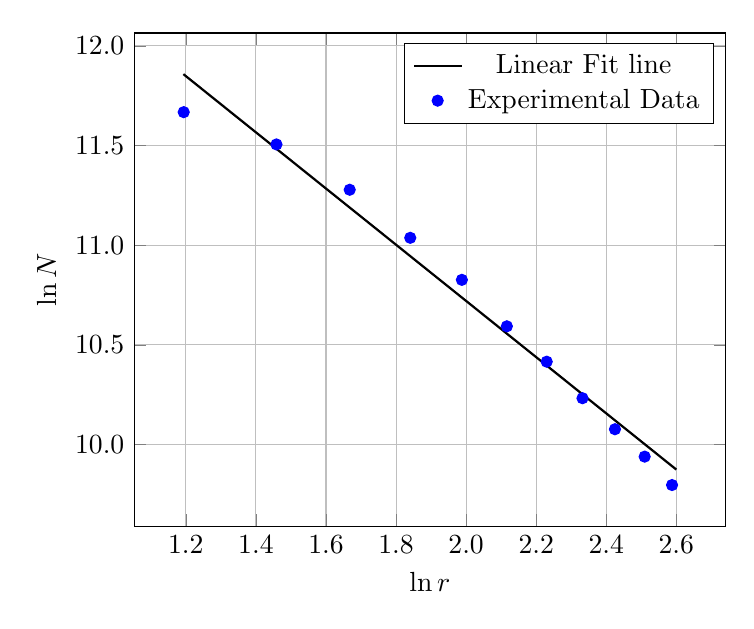
\begin{tikzpicture}
		\begin{axis}[grid,x tick label style={/pgf/number format/.cd, fixed, fixed zerofill, precision=1,/tikz/.cd},y tick label style={/pgf/number format/.cd, fixed, fixed zerofill, precision=1,/tikz/.cd}, xlabel = {$ \ln r $}, ylabel={$ \ln N $},width=0.75\linewidth]
			\addplot[domain=1.193:2.6, thick, smooth, no markers] {-1.41*x + 13.54};
			\addlegendentry{Linear Fit line}
			
			%			\addplot[only marks] file {1201-data.txt};
			\addplot[only marks,blue] coordinates {
				(1.193922468,11.667139)
				(1.458615023,11.50528636)
				(1.667706821,11.27782741)
				(1.840549633,11.03675352)
				(1.987874348,10.8258465)
				(2.116255515,10.59274384)
				(2.2300144,10.41524274)
				(2.332143895,10.23208362)
				(2.424802726,10.07645999)
				(2.509599262,9.938935131)
				(2.587764035,9.79645898)
			};
			\addlegendentry{Experimental Data};
		\end{axis}
	\end{tikzpicture}
	\caption{Plot of $ \ln N $ versus $ \ln r $ ; The slope of the least-square fit line is $ -1.41 $ units, and $ y $-intercept is $ 13.54 $ units.}
	\label{fig:lnN-lnr}
\end{figure}
%The plot of $ \ln r $ versus $\ln N $ is shown in the figure \ref{fig:my_label}
%	\begin{figure} [!htb]
%	    \centering
%	    \includegraphics[width=0.7\textwidth]{Experiments/inverse square law new.PNG}
%	    \caption{Plot of $\ln r $ versus $\ln N$}
%	    \label{fig:my_label}
%	\end{figure}
	
	\section{Result}
	The inverse square law has been verified for gamma particles.
	\clearpage
	
\end{document}